% !TEX program = xelatex
\documentclass[11pt,a4paper]{article}
\usepackage[numbers,sort&compress]{natbib}
\usepackage{geometry}
\usepackage{fontspec} 
\usepackage{underscore}
\usepackage{graphicx} 
\usepackage{hyperref}
\usepackage{multicol}
\usepackage{multirow}
\usepackage{parskip}
\usepackage{booktabs}
\usepackage{float}
\usepackage{subfigure}
% insert code
\usepackage{color}
\usepackage{listings}
\usepackage{setspace}
\definecolor{Code}{rgb}{0,0,0}
\definecolor{Decorators}{rgb}{0.5,0.5,0.5}
\definecolor{Numbers}{rgb}{0.5,0,0}
\definecolor{MatchingBrackets}{rgb}{0.25,0.5,0.5}
\definecolor{Keywords}{rgb}{0,0,1}
\definecolor{self}{rgb}{0,0,0}
\definecolor{Strings}{rgb}{0,0.63,0}
\definecolor{Comments}{rgb}{0,0.63,1}
\definecolor{Backquotes}{rgb}{0,0,0}
\definecolor{Classname}{rgb}{0,0,0}
\definecolor{FunctionName}{rgb}{0,0,0}
\definecolor{Operators}{rgb}{0,0,0}
\definecolor{Background}{rgb}{0.98,0.98,0.98}
\lstdefinelanguage{Python}{
numbers=left,
numberstyle=\footnotesize,
numbersep=1em,
xleftmargin=1em,
framextopmargin=2em,
framexbottommargin=2em,
showspaces=false,
showtabs=false,
showstringspaces=false,
frame=l,
tabsize=4,
% Basic
basicstyle=\ttfamily\small\setstretch{1},
backgroundcolor=\color{Background},
% Comments
commentstyle=\color{Comments}\slshape,
% Strings
stringstyle=\color{Strings},
morecomment=[s][\color{Strings}]{"""}{"""},
morecomment=[s][\color{Strings}]{'''}{'''},
% keywords
morekeywords={import,from,class,def,for,while,if,is,in,elif,else,not,and,or,print,break,continue,return,True,False,None,access,as,,del,except,exec,finally,global,import,lambda,pass,print,raise,try,assert},
keywordstyle={\color{Keywords}\bfseries},
% additional keywords
morekeywords={[2]@invariant,pylab,numpy,np,scipy,itertools,cycle,matplotlib,pyplot,plt,os,listdir,cv2,sklearn,metrics,roc_curve,auc},
keywordstyle={[2]\color{Decorators}\slshape},
emph={self},
emphstyle={\color{self}\slshape},}
%
\newfontfamily\cc{Courier} %font for all code related things
\setmainfont{Times New Roman}
\author{
    Su Jia Yin\\
    UW ID: sjyin\\
    sjyin@uwaterloo.ca
    \and
    Alyssa Yiqin Huang\\
    UW ID: y672huan\\
    y672huan@uwaterloo.ca
    \and
    Dawson(Xiaohui) Men\\
    UW ID: xmen\\
    xmen@uwaterloo.ca
}
\geometry{letterpaper,scale=0.7}
\title{Enhancements to Gramfuzz, a Grammar-based Fuzzing Tool}
%%%%%%%%%

\begin{document}
\setlength{\parskip}{1em} 
\setlength{\parindent}{2em}
\maketitle
%%%%%%%%%%%%

\begin{abstract}
    We enhanced {\cc gramfuzz}, a grammar-based fuzzing tool, by designed a runner program to select the program-under-test and its grammar, feed the inputs automatically, save suspicious inputs and display the testing status in an interface. Compared to the mutation-based fuzzing tool, our enhanced grammar-based fuzzing tool penetrates deeper into benchmarks' parsers. 
\end{abstract}

%------------------------------------------------------
% Introduction:
% Briefly state the problem you are solving
% Why is it important and interesting
% Why other methods may not work for this problem
% Briefly describe your method and why it is better than previous methods
\section{Introduction}
It is difficult to explore unexpected or abnormal behaviour in software engineering, especially for closed source software.\cite{fuzzingbook2020}  Due to the complexity of software, it is almost unavoidable that several errors or exceptions, which may lead to economic loss or even security and safety problems, occurs in a piece of software. As Paul Strassman commented, software easily rates as the most poorly constructed, unreliable, and least maintainable technological artifacts invented by man. Thus, it is important to test a piece of software before it is used as a system component. It is also interesting to find out what kind of inputs could trigger the software-under-test to crash.

When we can not access the source codes or I/O behaviours of the target software, it is impossible to use gray-boxed or white-boxed methods, including static analysis or concolic testing. Thus, though with several disadvantages, black-box testing methods, such as fuzzing, are necessary. Among all kinds of black-box fuzzing methods, the grammar-based fuzzing method is very suitable for the scenario of using closed source software as system components. As known to be an effective technique for checking security vulnerabilities in programs, grammar-based fuzzer generates well-formatted inputs by specifying inputs via the grammar of the program-under-test. \cite{8636353,7958599}. Furthermore, the application programming interface and the input format generated by other programs are already known, which limits the formats and range of inputs and decreases the cost of writing grammars.

As we noticed, most of the grammar-based fuzzing tools require the users to input the generated files to the program-under-test manually, which would be extremely inefficient when there are thousands of test cases. Thus, we designed a runner program to feed the inputs generated by fuzzer into the program-under-test automatically and display the current status with an interface.

%------------------------------------------------------
% Description of your method/algorithm:
% Clearly describe your algorithm (ideally in algorithmx format available in MS Word and Latex with line numbers)
% It would be great if you can provide a complexity-theoretic analysis of your algorithm
\section{Description of the method}
\subsection{Framework or tool chain used}
\subsubsection{Fuzzing tools}
We choose \href{https://d0c-s4vage.github.io/gramfuzz/}{\cc gramfuzz}, a open-source grammar-based fuzzing Python library, to write the grammars for benchmarks and designed an input generator. As comparision, we choose \href{https://pypi.org/project/pyZZUF/}{\cc pyZZUF}, a Python library implements bit-flip zzuf mutator, to generate inputs according to a random inputs generated by {\cc gramfuzz}. 
%
\subsubsection{Runner program}
To increase the efficiency of fuzzing test, we designed a runner program. As Fig. \ref{ui} shows, the interface of the runner program allows the user to choose the fuzzer, benchmark, input type (feed), timeout. Also, the user can select how many input files will be generated and feed to the benchamrk in a single round and how many rounds will be executed. 
\begin{figure}[H]
    \centering
    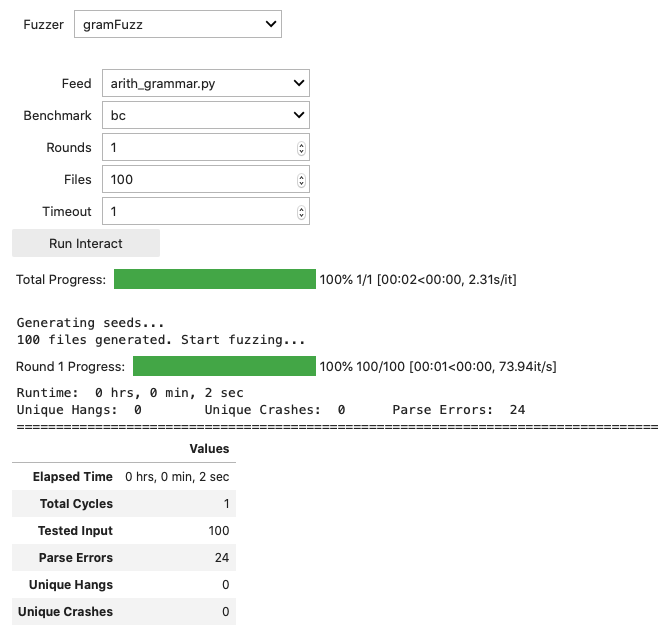
\includegraphics[width=0.5\textwidth]{ui.png}
    \caption{Interface of runner program}
    \label{ui}
\end{figure}

%
\subsection{Benchmarks used}
We chose two calculators as benchmarks. One is \href{https://www.gnu.org/software/bc/manual/html_mono/bc.html}{\cc bc}, another one is \href{https://www.systutorials.com/docs/linux/man/1-calc/}{\cc calc}. 
Both two programs are command-line programs, and their input formats are also similar to each other. Therefore, it would be clear to illustrate the strength of grammar-based fuzzing that it can decrease the possibility of the inputs rejected by the parser and penetrate more in-depth than other fuzzing methods by generating well-formatted inputs.

Furthermore, {\cc bc} and {\cc calc} could be considered as representative of program-under-test, because their inputs can be divided into two types, one type is the arithmetical calculation, and the other type is program statement, including defining or calling functions, if-else conditional branchings, for loops and while loops. Thus, these two benchmarks are very typical, which makes the results have general meanings.
%
\subsection{Grammar designed}
We noticed that the average execution time for two benchmarks is significantly longer when the input is arithmetical calculation. It is because that big numbers and complicated calculations, such as exponent arithmetic, will trigger long-running uninterruptible computation.
Since we detected the program hang by setting a timeout, we designed grammar for arithmetical calculation inputs and program statement inputs separately. Thus, we could set a longer timeout for arithmetical calculation when running the test. As for mutation-based fuzzer, we used seed inputs generated by the grammar-based fuzzer according to specific grammars to mutate and generate inputs for the specific type of inputs. 
%------------------------------------------------------
% Results
% Describe your benchmarks and experimental setup (i.e., what kind of machines, OS, compiler used etc...)
% Compare your tool against some naive approach and show why it is better (e.g., random fuzzing)
% Use graphs and charts to describe your experimental result
\section{Results}
\subsection{Experimental setup}
We run the testing on Mac OS X. Table \ref{setup} shows the version of software or library we used.
\begin{table}[H]
    \centering
    \label{setup}
    \caption{Experimental setup}
    \begin{tabular}{c c c}
        \toprule
        Software/Library & $\quad$& Version\\
        \midrule
        {\cc gramfuzz} & $\quad$& 1.14.0\\
        {\cc pyZZUF} & $\quad$& 0.1\\
        {\cc bc} & $\quad$& 1.06\\
        {\cc calc} & $\quad$& 2.12.7.1\\
        Python & $\quad$& 3.7.6\\
        \bottomrule
    \end{tabular}
\end{table}

\subsection{Experimental result}
Table \ref{result} shows the experimental results. We found crashes when using {\cc gramfuzz} to test {\cc bc} with program statement inputs. The crashes were triggered by segment fault.
\begin{table}[H]
    \centering
    \label{result}
    \caption{Experimental result for 100000 tested inputs}
    \begin{tabular}{ccccccc}
        \toprule
        Fuzzer & Benchmark & Input type  & Parser errors & Hang & Crash & Duration\\
        \midrule
        \multirow{4}{*}{\cc bc}& \multirow{2}{*}{Arithmetic} 
        & {\cc gramfuzz} & 19045 & 0 & 0 & 00:30:52\\
        \cline{3-7}
        & & {\cc pyZZUF} & 50000 & 50000 & 0 & 14:10:24\\
        \cline{2-7}
        & \multirow{2}{*}{Statement} 
        & {\cc gramfuzz} & 9449 & 0 & 24 & 00:27:17\\
        \cline{3-7}
        & & {\cc pyZZUF} & 100000 & 0 & 0 & 00:51:06\\
        \midrule
        \multirow{4}{*}{\cc calc}& \multirow{2}{*}{Arithmetic} 
        & {\cc gramfuzz} & 0 & 0 & 0 & 00:35:59\\
        \cline{3-7}
        & & {\cc pyZZUF} & 50000 & 50000 & 0 & 14:23:54\\
        \cline{2-7}
        & \multirow{2}{*}{Statement} 
        & {\cc gramfuzz} & 99745 & 0 & 0 & 00:47:46\\
        \cline{3-7}
        & & {\cc pyZZUF} & 100000 & 0 & 0 & 00:52:36\\
        \bottomrule
    \end{tabular}
\end{table}
Compared {\cc gramfuzz} to {\cc pyZZUF} according to the data in Table \ref{result}, the results are presented as Fig. \ref{duration} and Fig. \ref{result-comp}. From Fig. \ref{duration}, we can concluded that it took more time to test 100 thousands input files at any cases, especially when the input tpye is arithmetic calculation.
From Fig. \ref{result-comp}, we could see that the inputs generated by {\cc gramfuzz} were significantly less likely to be rejected by the parser than inputs generated by {\cc pyZZUF}, regardless of the benchamrk and the input type.
\begin{figure}[H]
    \centering
    \label{duration}
    
    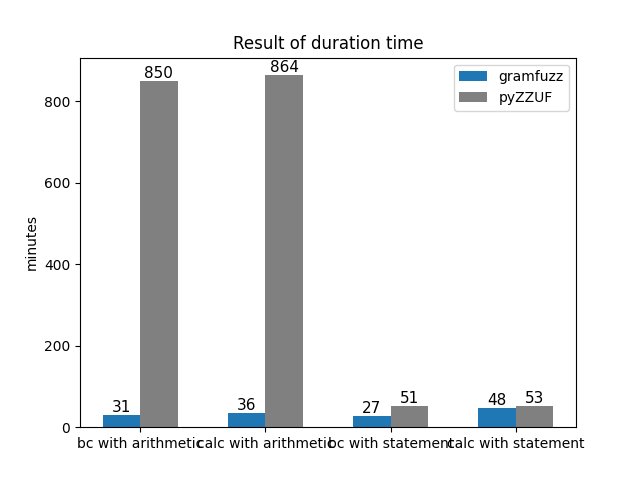
\includegraphics[width=0.6\textwidth]{duration.png}
    \caption{Duration time for testing 100000 inputs file}
\end{figure}


\begin{figure}[H]
    \centering   
    \label{result-comp}
    \subfigure[{\cc bc} with arithmetic calculation inputs]{
        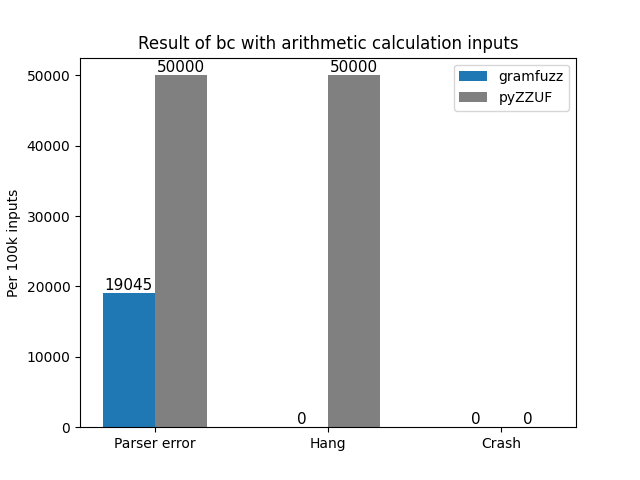
\includegraphics[width=0.4\textwidth]{bc-arith.png}}
   \subfigure[{\cc bc} with program statement inputs]{
        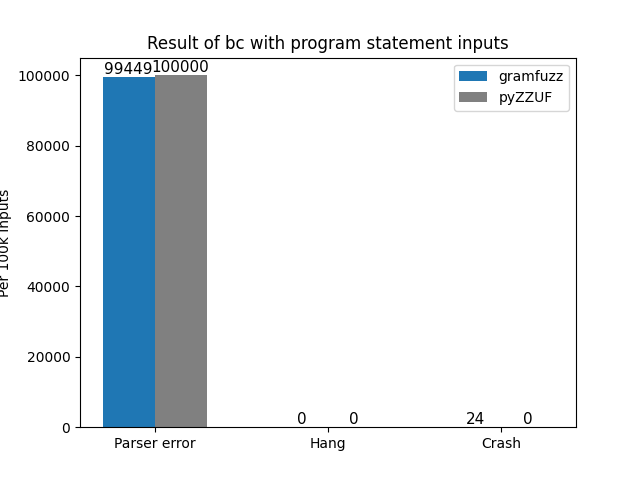
\includegraphics[width=0.4\textwidth]{bc-state.png}}

    \subfigure[{\cc calc} with arithmetic calculation inputs]{
        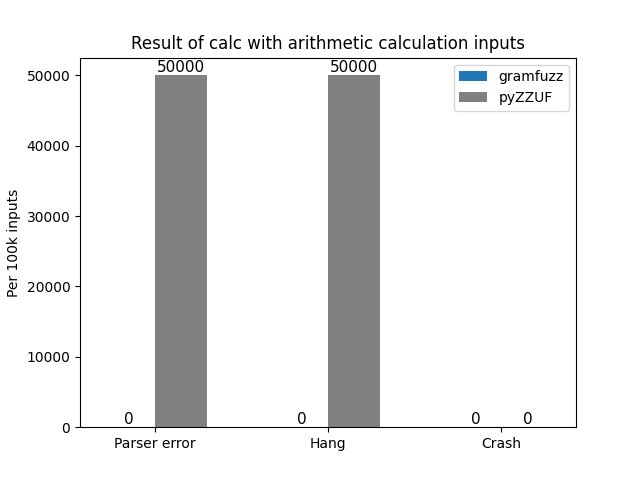
\includegraphics[width=0.4\textwidth]{calc-arith.png}}
   \subfigure[{\cc calc} with program statement inputs]{
        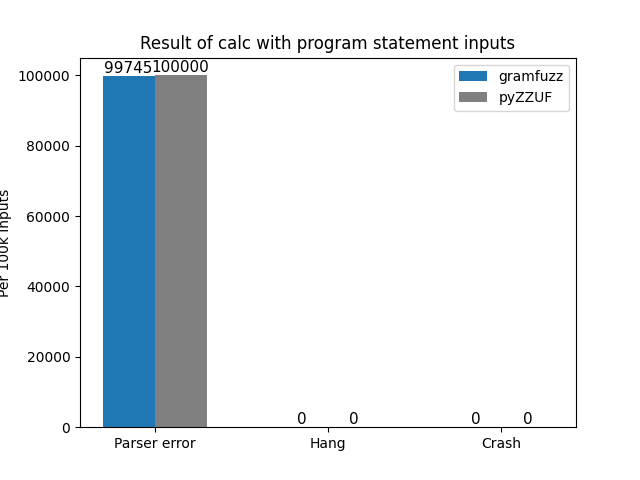
\includegraphics[width=0.4\textwidth]{calc-state.png}}
    \caption{Results compared {\cc gramfuzz} to {\cc pyZZUF}}    
\end{figure}

%------------------------------------------------------
% Conclusions and future work
% Describe your conclusions and next steps if you were to continue the project
\section{Conclusions and future work}
\subsection{Conclusions}

\subsection{Future work}


\bibliography{proposal}
\bibliographystyle{plain} 
\end{document}